\documentclass[12pt]{article}
\usepackage[utf8]{inputenc}
\usepackage{graphicx}
\usepackage{array}
\usepackage[english]{babel}
\usepackage{float}
\usepackage[colorlinks,linkcolor=black,bookmarksopen,bookmarksnumbered,backref]{hyperref}
\usepackage{multirow}
\usepackage[x11names,rgb,table,xcdraw]{xcolor}
\usepackage{listings}
\usepackage[a4paper]{geometry}
\usepackage[acronym]{glossaries}

\newcommand{\aqnote}[1]{ {\color{violet}\textbf{AQ:} #1 } }

\newacronym{hpc}{HPC}{High Performance Computing}
\newacronym{isa}{ISA}{Instruction Set Architecture}
\newacronym{fpga}{FPGA}{Field Programmable Gate Array}
\newacronym{lut}{LUT}{Lock-Up Table}
\newacronym{dsp}{DSP}{Digital Signal Processors}
\newacronym{tlp}{TLP}{Transaction Layer Packet}
\newacronym{axi}{AXI-ST}{AXI4-Stream}
\newacronym{ip}{IP}{Intellectual Property}
\newacronym{vpu}{VPU}{Vector Processor Unit}
\newacronym{rtl}{RTL}{Register-Transfer Level}
\newacronym{dw}{Dword}{Double word}
\newacronym{hdl}{HDL}{Hardware Description Language}


\newacronym{epi}{EPI}{European Processor Iniciative}

\newacronym{io}{IO}{input/ouput}



\lstset{
  language=Verilog,
  basicstyle=\ttfamily\small, 
  keywordstyle=\color{purple}\bfseries,
  stringstyle=\color{red},
  commentstyle=\color{blue},
  morecomment=[s][\color{blue}]{/**}{*/},
  extendedchars=true, 
  showspaces=false, 
  showstringspaces=false, 
  numbers=left,
  numberstyle=\scriptsize,
  breaklines=true, 
  backgroundcolor=\color{cyan!3}, 
  breakautoindent=true, 
  captionpos=b,
  xleftmargin=0pt,
  tabsize=4,
  frame=single
}

\setlength{\parindent}{2em}
\setlength{\parskip}{0.5em}

\title{RISCV processor in an \acrshort{fpga}}
\author{Jose Luís Estragués \\ Andrea Querol \\ Guillem Ramírez \\ Joan Vinyals \\ Pablo Vizcaíno}
\date{May 2021}
% \institute[FIB, UPC]{Facultat d'Informàtica de Barcelona \\ Universitat Politècnica de Catalunya - BarcelonaTech \and Barcelona Supercomputing Center}

\begin{document}
\makeatletter

\begin{titlepage}
\thispagestyle{empty}
\begin{center}
	\centering
	\vspace{1cm}
	{\scshape\Large MA - Multiprocessor Architecture  \par}
	\vspace{0.75cm}
	{\Large Course 2020/21 \par}
	\vspace{0.75cm} 
	{\huge\bfseries RISC-V processor in an \acrshort{fpga} \par}
	\vspace{1cm}
	{\Large Jose L. Estragués \par  Andrea Querol \par  Guillem Ramírez \par  Joan Vinyals \par  Pablo Vizcaino}
	\vspace{1cm}
    \vspace{0.5cm}
    

 \vfill
% Bottom of the page
	{\large 22 June, 2021\par}
\end{center}


\clearpage
\end{titlepage}



\tableofcontents


\section{RISC-V}

RISC-V is an open standard instruction set architecture (\gls{isa}) based in the reduced instruction set computer (\gls{risc}) architecture. This architecture is based on a small and highly optimized instructions in contrast with other types of architectures like the complex instruction set computer (\gls{cisc}). The RISC-V \gls{isa} does not need fees to use and several companies and projects  are considering this architecture to develop their products. In addition, open source operating systems with RISC-V support are available and the instruction set is supported in several popular software toolchains. Load-store architecture and IEEE-754 floating point instructions. \\

\subsection{History}

Prof. Krste Asanović and graduate students Yunsup Lee and Andrew Waterman started the RISC-V instruction set in May 2010 \cite{riscvh} as part of the Parallel Computing Laboratory (Par Lab) at UC Berkeley, California. The initial purpose of the RISC - V was to offer an open source hardware that could be used for academic purposes and it could be deployable in any hardware or software design without royalties.\\

The architecture has as a precedent the DLX MIPS instruction set by David Patterson. David Patterson joined the project and was the originator of the Berkeley RISC. RISC-V is the fifth generation of a series of cooperative RISC-based research projects. The authors and their institutions originally sourced the ISA documents and several CPU designs which would allow derivative work to be rather open and free or close and property. The \gls{isa} specification was published in 2011  with all rights reserved. \\

RISC-V foundation was created to own, maintain, and publish intellectual property related to RISC-V's definition. Commercial users needed a stable \gls{isa} to develop products that would be used for years. For this reason, the authors and owners had to give their rights to the foundation. The foundation moved from US to Switzerland concerning the US trade conditions in 2019. Its named changed to RISC-V International and since then they have freely published the documents defining RISC-V and permits unrestricted use of the \gls{isa} for design of software and hardware. However, changes can only be accepted by the members of the foundation. \\

\subsection{\gls{isa} base and extensions} 
One of the more interesting characteristics about RISC-V is the popularity and this is reflected in the \gls{isa} extensions that consist in alternative base and optional extensions. The base can implement a simplified general-purpose computer including compilers. It specifies: 

\begin{itemize}
	\item Instructions and their encoding
	\item Control flow
	\item Registers and their size
	\item Memory and addressing
	\item Logic manipulation
\end{itemize}

In table \ref{tab:isa}, the \gls{isa} modules are listed and described:

\begin{table}[H]
\centering
\begin{tabular}{|c|c|c|c|}
\hline
\textbf{Name} & \textbf{Description} & \textbf{Status}  & \textbf{Ins. Count}  \\ \hline

\multicolumn{4}{|c|}{\textbf{\gls{isa} base}} \\ \hline
RVWMO & Weak Memory Ordering & Ratified & \\ \hline
RV32I & Base Integer Instruction set (32 bits) & Ratified & 49 \\ \hline
RV32E & Base Integer Instruction set embedded & Open & 49 \\ \hline
RV64I & Base Integer Instruction set (64 bits) & Ratified & 14 \\ \hline
RV128I & Base Integer Instruction set (128 bits) & Open & 14 \\ \hline

\multicolumn{4}{|c|}{\textbf{\gls{isa} extensions}} \\ \hline

M & Multiplication Division & Ratified & 8\\ \hline
A & Atomic Instruction & Ratified & 11 \\ \hline
F & Single precision FP & Ratified & 25 \\ \hline
D & Double precision FP & Ratified & 25 \\ \hline
Q & Quad precision FP & Ratified & 27 \\ \hline
C & Compressed Instruction & Ratified & 36 \\ \hline
Zicsr & Control and Status Register (CSR) & Ratified &  \\ \hline
Zifencei & Instruction-Fetch Fence & Ratified & \\ \hline
\end{tabular}
\caption{RISC-V popular \gls{isa} modules.} Reproduced from \cite{riscvg}.
\label{tab:isa}
\end{table}

Required \gls{isa} modules it is a characteristic to evaluate possible RISC-V cores depending on the functionalities the developers want to offer.

\subsection{Registers}
RISC-V cores typically have 32 integer registers and 32 floating-point registers when this extension is implemented. Each register has its functionality that is a consensus of the RISC-V developers. This is the method to keep information consistent and meaningful. In \ref{tab:riscreg} we can see the registers' convention.


\begin{table}[H]
\centering
\begin{tabular}{|c|c|c|c|}
\hline
\textbf{Register name} & \textbf{Symbolic name} & \textbf{Description}  & \textbf{Saved By}  \\ \hline
\multicolumn{4}{|c|}{\textbf{Integer registers}} \\ \hline
x0 & Zero & Always zero & \\ \hline
x1 & ra & Return address & Caller \\ \hline
x2 & sp & Stack Pointer & Callee \\ \hline
x3 & gp & Global pointer &  \\ \hline
x4 & tp & Thread pointer & Caller \\ \hline
x5 & t0 & Temporary/ alternate return address & Caller \\ \hline
x6-7 & t1-2  & Temporary & Caller \\ \hline
x8 & s0/fp & Saved register/ frame pointer & Callee \\ \hline
x9 & s1 & Saved register & Callee \\ \hline
x10-11 & a0-1 & Function argument/ return value & Caller \\ \hline
x12-17 & a2-7 & Function argument & Caller \\ \hline
x18-27 & s2-11 & Saved register & Callee \\ \hline
x28-31 & t3-6 & Temporary & Caller \\ \hline
\multicolumn{4}{|c|}{\textbf{Floating-point extension registers}} \\ \hline
f0-7 & ft0-7 & Floating-point temporaries & Caller \\ \hline
f8-9 & fs0-1 & Floating-point saved & Callee \\ \hline
f10-11 & fa0-1 & Floating-point arg/ return value & Caller \\ \hline
f12-17 & fa2-7 & Floating-point arg & Caller \\ \hline
f18-27 & fs2-11 & Floating-point saved registers & Callee \\ \hline
f28-31 & ft8-11 & Floating-point temporaries & Caller \\ \hline
\end{tabular}
\caption{RISC-V registers.} Reproduced from \cite{riscvg}.
\label{tab:riscreg}
\end{table}

Basically, certain registers will be used depending on the role of the value that they will store. Temporary registers are used to store and work with values that we don't need after a function call. Saved registers will store the values that are relevant to save during the function calls.  Certain registers are also predefined to pass arguments, return values and stack pointers which helps with data consistency. Symbolic name is used to a more user-friendly assembler code. 




\section{\gls{fpga}}



\section{RISC-V Cores}

\subsection{Selection criteria}
The first step for developing the project is to select a suitable riscv implementation. Therefore, we defined the following guidelines for the decision:
\begin{itemize}
\item Multicore capable design.
\item Open or accessible design.
\item The resource usage of the core must fit the capabilities of our FPGA. In addition, we must take into account that we are aiming for a multicore target. Therefore, resource usage is critical.
\item Maximize the compatibility with our \gls{fpga}. Each \gls{fpga} has its own devices and peripherals such as memory, clock, and ports. Hence we should look for designs that are well integrated with our device to ease the deployment of the core into our \gls{fpga}.
\item As the project aims to boot something, we thought of finding a design that can boot Linux.
\end{itemize}

\subsection{Ariane}
Ariane is a 6 stage CPU initially developed at ETH Zurich. It fully supports I, A, M and C extensions which enable the core to boot Linux.

The standalone design cannot be multicore. However, Openpiton enables the design to be multicore. Openpiton\cite{openpiton} is an Open Source framework for building scalable architecture research prototypes from 1 to 500 million cores.

Figure \ref{fig:openpitonariane} shows the proposed architecture by OpenPiton designers. First, each Ariane core has its L1 cache and then an adapter for the OpenPiton cache. Next, a P-Mesh controller is attached to each core with an additional cache (L1.5), routing and a shared and distributed L2 cache with a directory-based coherence protocol. Then a 2D-mesh is formed with the tiles (P-mesh controller + Ariane core). 

\begin{figure}[h]
    \centering
    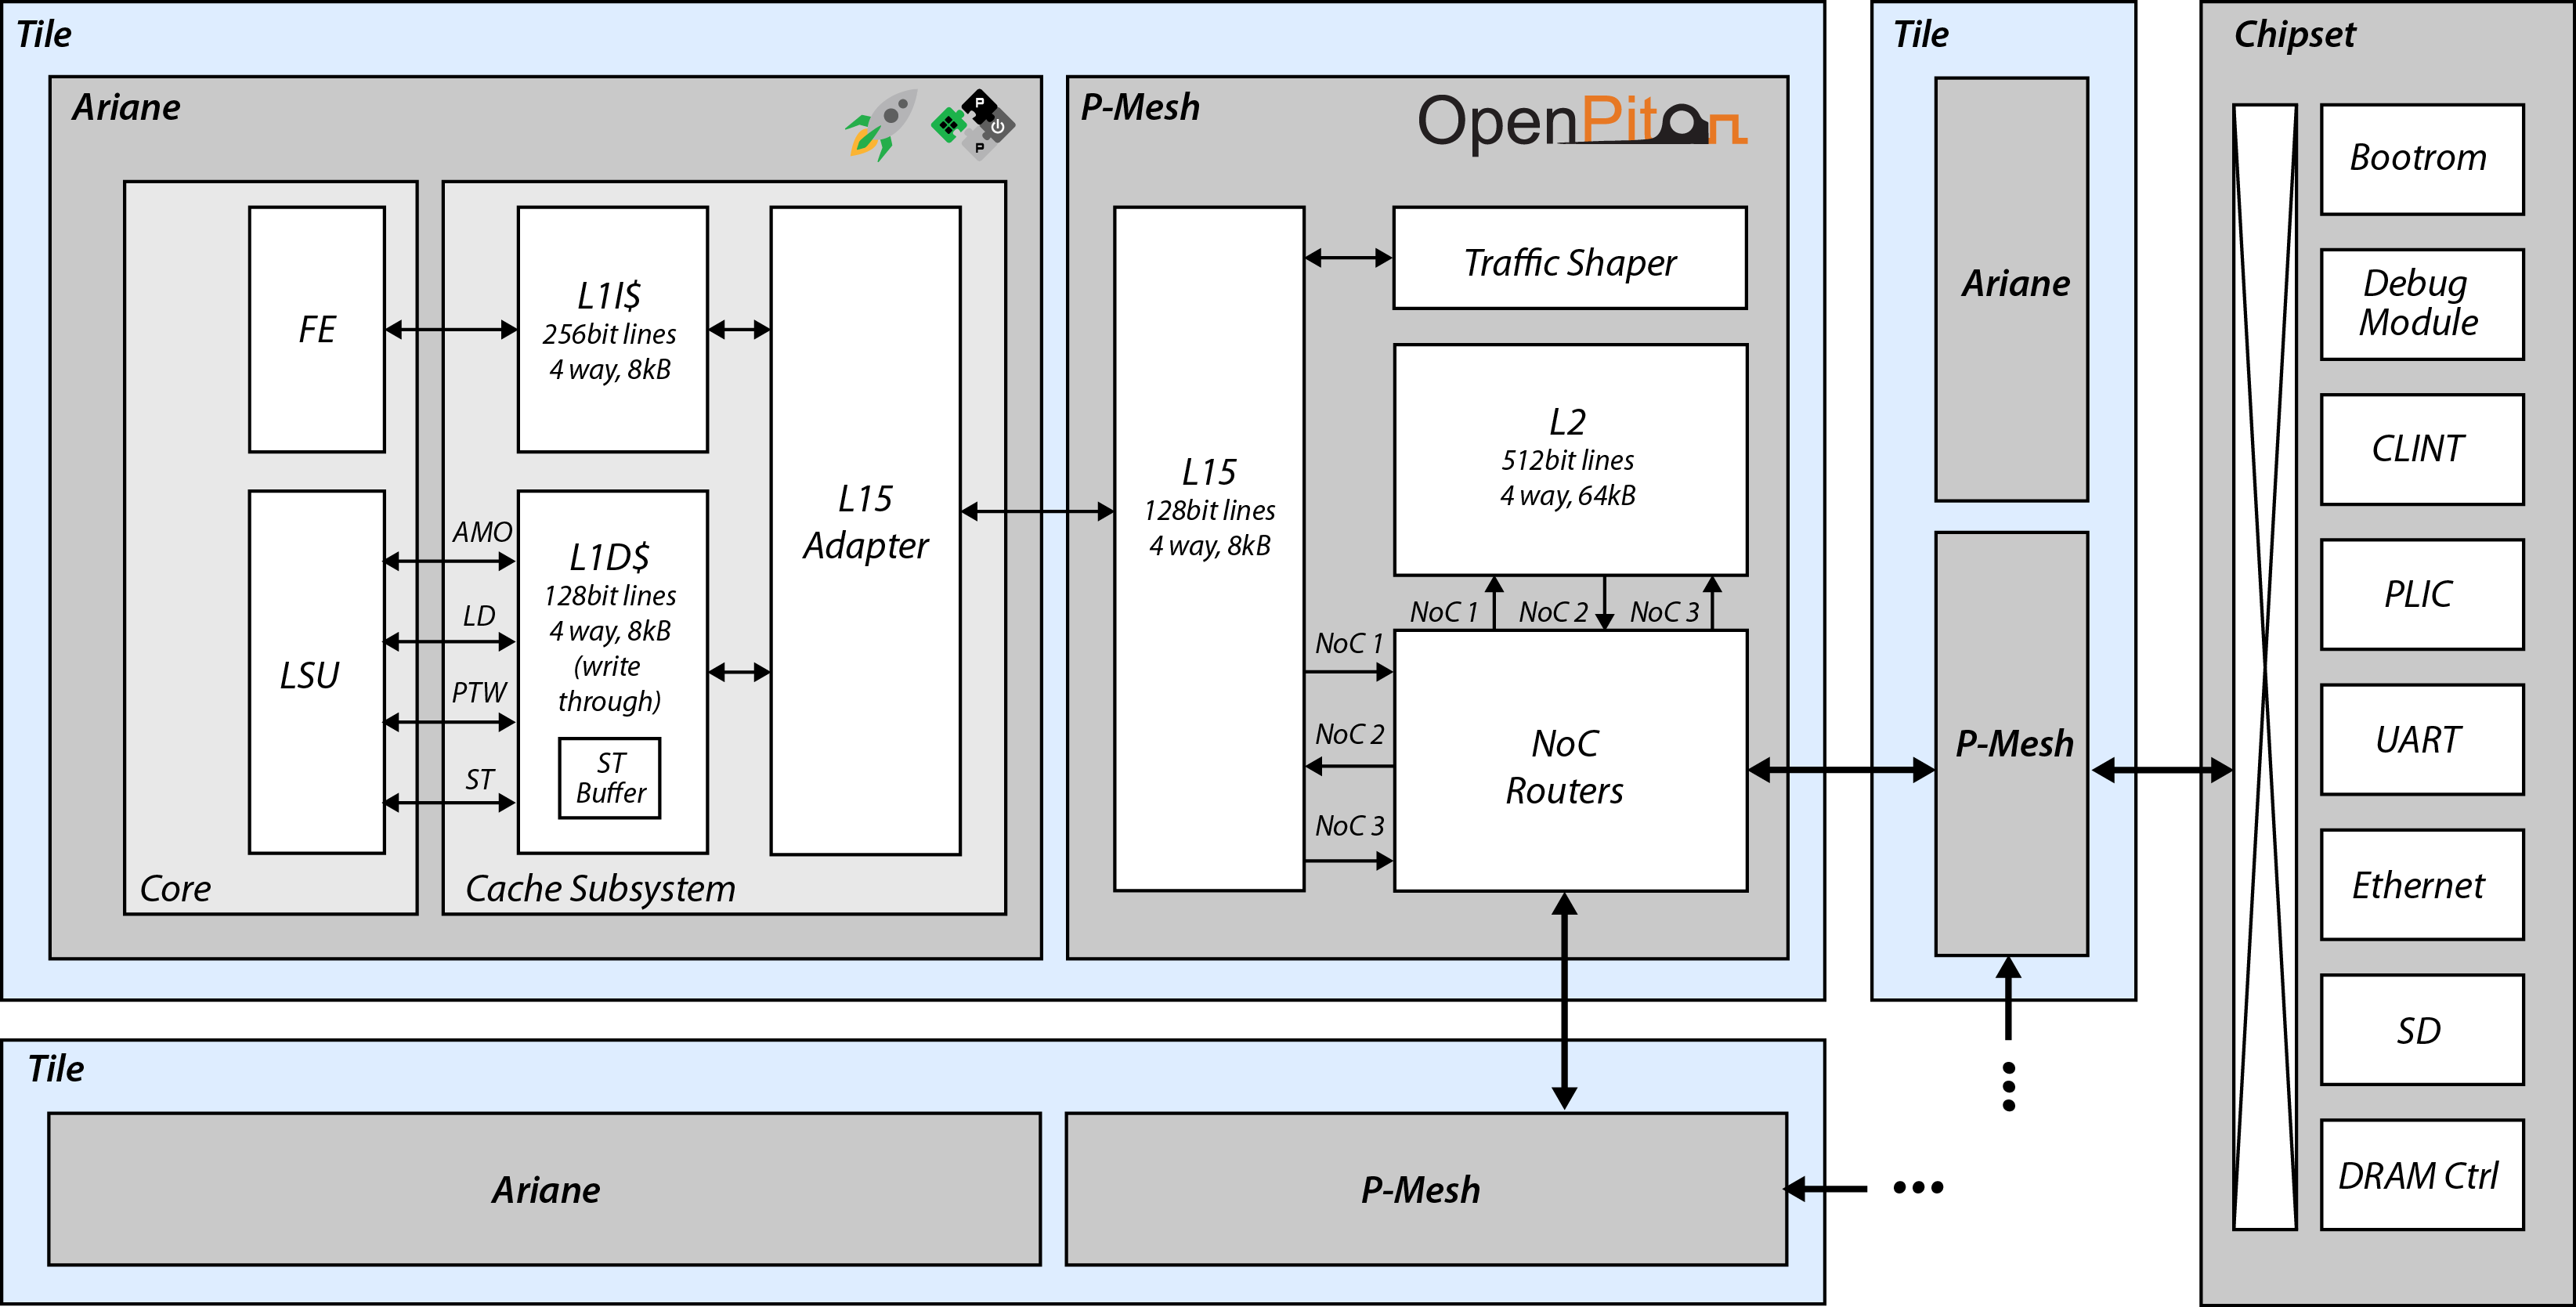
\includegraphics[width=0.9\textwidth]{img/openpiton_ariane_blockdiag.png}
    \caption{Openpiton and ariane block diagram.}
    \label{fig:openpitonariane}
\end{figure}

The main issue we encountered when trying to deploy the core was generating the bitstream. The design only officially supports the "Genesys2", "Nexys Video", and "VC707" boards. We tried to port and adapt it to our board, but we could not manage to do it. We decided to try another core because of the considerable complexity of the project and the knowledge needed to make the portability to our board possible.

\subsection{Rocketchip}
Rocketchip is a \gls{soc} generator designed at the University of Berkeley, California \cite{rocket}. From a configuration, it generates the full implementation, including multiple cores, caches and coherence protocol. It uses Chisel\footnote{\url{https://github.com/chipsalliance/chisel3}} as \gls{hdl}, a Scala-based language for \gls{asic} and \gls{fpga} logic designs. It implements the RISCV64G \gls{isa} variant. It is capable of booting Linux and allow different multicore configurations.

Figure \ref{fig:rocketstruct} shows \gls{soc} structure. The Rocketchip uses Rocket, BOOM or Zscale cores as a basic unit. Each core has its L1 data and instruction caches and a RoCC coprocessor. These units (Tiles) are interconnected using Tilelink, which interconnects the tiles with the level two cache. Tilelink is flexible and allows different cache coherence protocols. Finally, an AXI4 bridge connects the Tilelink module with the AXI4 crossbar, enabling the cores to access various devices and peripherals such as the \gls{dram}, IO devices.

\begin{figure}[h]
  \centering
  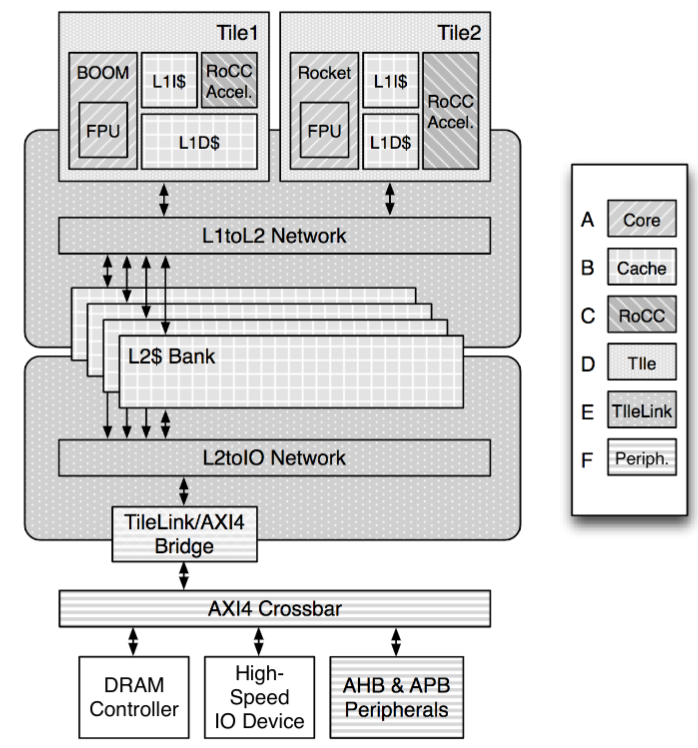
\includegraphics[width=0.6\textwidth]{images/rocket_structure.png}
  \caption{Rocketchip \gls{soc} structure}
  \label{fig:rocketstruct}
\end{figure}

When trying to deploy the Rocketchip \gls{soc}, we found out many difficulties. In particular, the lack of documentation, the Scala-based configuration and the resource usage made the deployment impossible.

\subsection{Darkriscv}
From the previous experience, we decided to take a different approach. We looked for a core that seems simple to deploy to our board and understand and then make the necessary modifications to accomplish project objectives.

Darkriscv\footnote{\url{https://github.com/darklife/darkriscv}} is a tiny and naive core that implements most of the RISCV32E and RISCV32I extensions. It uses few \gls{fpga} resources, and it has been tested on similar \gls{fpga} boards. The core is not designed to be multicore either to boot Linux. Therefore, we decided to rephrase the project objectives and defined new ones. First, to deploy Darkriscv into our \gls{fpga}, modify the design to be multicore capable, including a simple coherence system and boot simple programs to test the multicore design.

Its simplicity makes the design easy to understand, which enabled us to make the necessary modifications towards generating a bitstream for our \gls{fpga}.

Figure \ref{fig:bitstream_gen} illustrates the bitstream generation process. 
First, we create the Vivado project and import the source code files of Darkrsicv. Then we generate the constraints file, which maps between the hardware physical inputs and outputs to logical inputs and outputs for our code. In addition, we create the block design. Figure \ref{fig:block_design} shows the structure. We placed two blocks, a Xilinx Clock IP for our board and the Darksoc block, which contains the core. Then we connected the Xilinx clock to the Darksoc clock, the physical reset button to the core reset, the core LEDs to the board physical LEDs and the system clock to the Xilinx clocking IP.

\begin{figure}[h]
    \centering
    \begin{tikzpicture}[node distance=0.4cm]
      \node (prj) [stylepop] {Create Vivado project};
      \node (const) [stylepop, right=of prj ] {Design constraints file};
      \node (blk) [stylepop, right=of const] {Block design};
      \node (bit) [stylepop, right=of blk] {Generate bitstream};

      \draw [arrow] (prj) -- (const);
      \draw [arrow] (const) -- (blk);
      \draw [arrow] (blk) -- (bit);
    \end{tikzpicture}
    \caption{Bitstream generation process}
    \label{fig:bitstream_gen}
\end{figure}

\begin{figure}[h]
  \centering
  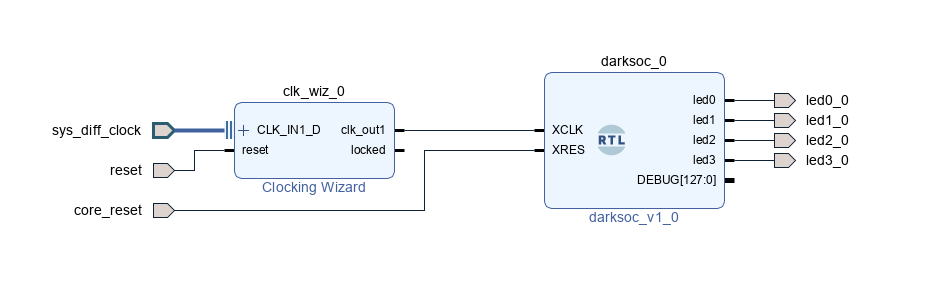
\includegraphics[width=0.8\textwidth]{../presentation/images/block-design.png}
  \caption{Darkriscv block design}
  \label{fig:block_design}
\end{figure}

Finally, once we have the block design, we are capable of synthesizing and generating the bitstream. 

\iffalse
[1] http://parallel.princeton.edu/openpiton/paper.html
[2] https://github.com/PrincetonUniversity/openpiton/blob/openpiton/docs/openpiton_ariane_blockdiag.png?raw=true
[3] https://www2.eecs.berkeley.edu/Pubs/TechRpts/2016/EECS-2016-17.html
[4] https://github.com/chipsalliance/chisel3
[5] Slides
[6] Slides

\fi

\section{Datapath}



\section{Referee}

%Justification
\subsection{Justification} \label{referee-justification}
Once we had defined the datapath of the core, we were ready to expand our single-core design into a multicore.
We can duplicate the datapath to generate as many cores as we desire. However, we will need to implement a shared memory design if we want them to communicate with each other through memory. 

Nevertheless, we cannot just create a single memory and connect all the cores to it. 
The original \textit{Darkriscv} design assumed an instantaneous memory that could complete read and write operations without delay, but we now have $N$ cores accessing the memory, so some will need to wait in the case of simultaneous accesses since we plan to serialize them.


%Behaviour
\subsection{Behaviour} \label{referee-behaviour}
We created a module calLED \textit{Referee}, which works as an interface between $N$ cores and the memory.
Its purpose is to grant access from the cores to the memory, halting the cores that must wait their turn to access it.
In a way, it acts as a single core from the memory side, so the memory is agnostic of the actual number of cores.
A simplified diagram of this module can be seen in Figure~\ref{referee-fig}.

\begin{figure}[h!]
    \centering
    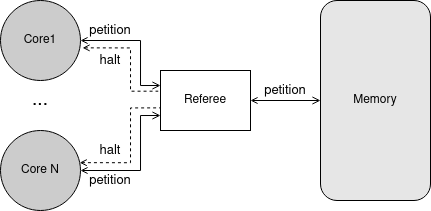
\includegraphics[width=.5\textwidth]{images/Referee_fig.png}
    \caption{Simplified diagram of the Referee.}
    \label{referee-fig}
\end{figure}

The \textit{Referee} treats read and write operations the same way.
For simplicity, we will refer to a \textit{petition} when we want to address both read and write operations.
If many cores send a petition at the same time, the \textit{Referee} chooses the one from the core with the highest ID, halts all the requesting cores, sends the petition to the memory, and waits for its answer.
If more cores try to access memory while an old petition is being served, the \textit{Referee} halts them.
When the memory finishes serving the petition, the core releases (unhalts) its associated core and serves the next petition.

%Verification
\subsection{Verification}
Once the module was designed, the next step was to test if it was working correctly.
In order to generate codes, we first write them with either assembly inline or C.
After that, we compile it with a modified \textit{gcc} supporting RISC-V found in the RISC-V Tools~\cite{tools} and then we use \textit{Objdump} to obtain the hexadecimal codification of the instructions.
This process is exemplified in Figure~\ref{coding}.

\begin{figure}[h!]
    \centering
    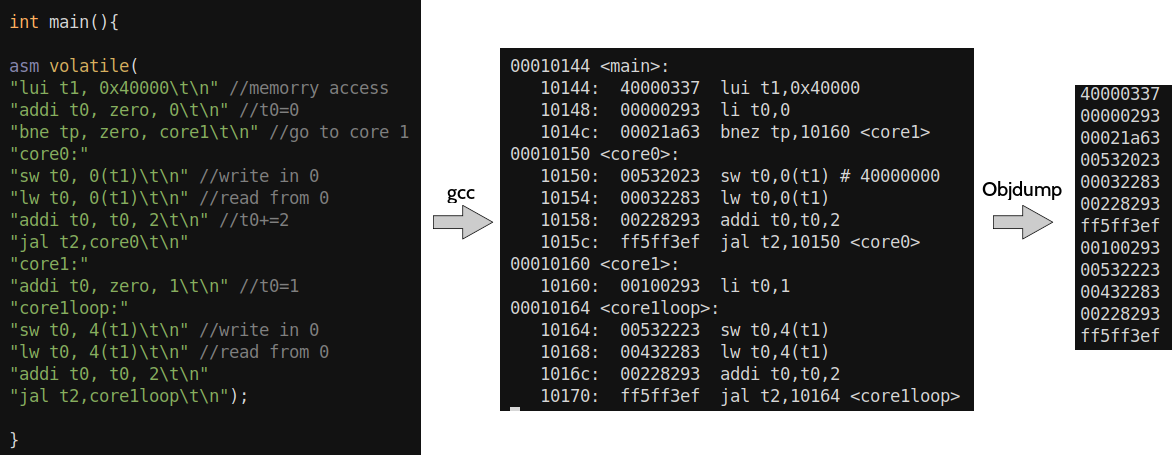
\includegraphics[width=.9\textwidth]{images/coding.png}
    \caption{Generating codes for Darkriscv.}
    \label{coding}
\end{figure}

Finally, the hexadecimal instructions are written in a file that acts as a ROM, embedded in the \gls{fpga} when generating the bitstream, or simply read when simulating.

The first test was to set the number of cores to 2 and run a straightforward code where they light up LEDs alternatively.



\begin{figure}[htbp]
\centering
\begin{minipage}[t][4cm][t]{4.5cm}
\textbf{Core 0}\\
while(1)\{\\
\hspace*{1cm}LEDs = [0 0 0 1];\\
\hspace*{1cm}flag0 = 1;\\
\hspace*{1cm}while(!flag1);\\
\hspace*{1cm}flag1 = 0;\\
\hspace*{1cm}LEDs = [0 1 0 0];\\
\}
\end{minipage}\hspace{2.5cm}
\begin{minipage}[t][4cm][t]{4.5cm}
\textbf{Core 1}\\
while(1)\{\\
\hspace*{1cm}while(!flag0);\\
\hspace*{1cm}flag0 = 0;\\
\hspace*{1cm}LEDs = [0 0 1 0];\\
\hspace*{1cm}flag1 = 1;\\
\}
\end{minipage}%
\vspace{.1cm}
\includegraphics[width=.75\textwidth]{images/LEDs2_fig.png}
\caption{Pseudocode of the test code with 2 processors.}
\label{2LED-code}
\end{figure}
\clearpage
In Figure~\ref{2LED-code} we can find the pseudocode that both cores are running and a scheme of the expected behaviour.
Core 0 lights up the first LED, signals core 1 to light up the second one and then to signal core 0 again to light up the third LED.

Figure~\ref{2LED-sim} shows the simulation of this code.
We see how core 0 lights up the first LED and waits some cycles before setting flag0 to 1, while core 1 repeatedly reads the value of this flag.
Then, the same happens, changing the roles of core 0 and core 1.

\begin{figure}[h!]
    \centering
    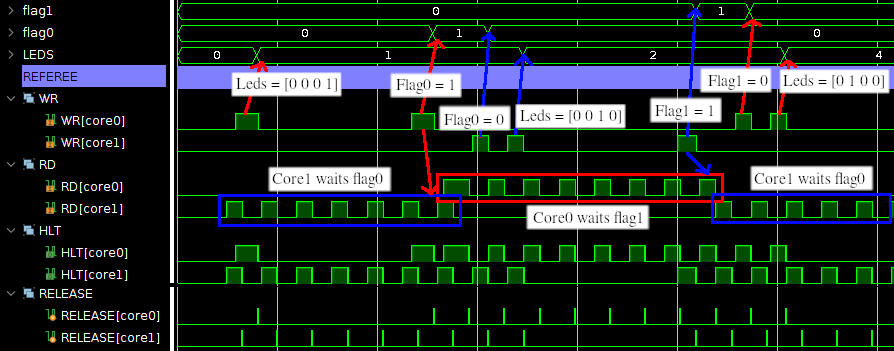
\includegraphics[width=1.0\textwidth]{images/flag2_sim_crop_arrows.png}
    \caption{Simulation of the code depicted in Figure~\ref{2LED-code}.}
    \label{2LED-sim}
\end{figure}


We can also zoom in to see an example of how the \textit{Referee} is working in this example. In Figure~\ref{2LED-close} we can see how core 0 tries to write while core 1 is waiting for the memory to complete a read petition.
The \textit{Referee} halts core 0 and does not send his petition until the read is finished.

\begin{figure}[h!]
    \centering
    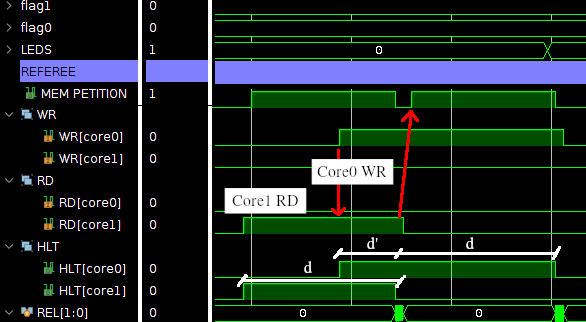
\includegraphics[width=0.7\textwidth]{images/flag2_sim_close_arrow.png}
    \caption{Simulation showing the serialitzation of memory accesses by the referee.}
    \label{2LED-close}
\end{figure}

Once we checked that this simple code was also working in the \gls{fpga}, we tried to complicate the design a little bit more.
We increased the number of cores from 2 to 4 and ran a very similar code, depicted in Figure~\ref{4LED-code}.
Core $i$ lights up LED $i$ and signals core $i+1$ to the same.

\begin{figure}[htbp]
\centering
\begin{minipage}[t][3cm][t]{3.2cm}
\textbf{Core 0}\\
while(1)\{\\
\hspace*{.4cm}while(flag!=0);\\
\hspace*{.4cm}LEDs=[0 0 0 1];\\
\hspace*{.4cm}flag=1;\\
\}
\end{minipage}\hspace{.5cm}
\begin{minipage}[t][3cm][t]{3.2cm}
\textbf{Core 1}\\
while(1)\{\\
\hspace*{.4cm}while(flag!=1);\\
\hspace*{.4cm}LEDs=[0 0 1 0];\\
\hspace*{.4cm}flag=2;\\
\}
\end{minipage}\hspace{.5cm}
\begin{minipage}[t][3cm][t]{3.2cm}
\textbf{Core 2}\\
while(1)\{\\
\hspace*{.4cm}while(flag!=2);\\
\hspace*{.4cm}LEDs=[0 1 0 0];\\
\hspace*{.4cm}flag=4;\\
\}
\end{minipage}\hspace{.5cm}
\begin{minipage}[t][3cm][t]{3.2cm}
\textbf{Core 3}\\
while(1)\{\\
\hspace*{.4cm}while(flag!=4);\\
\hspace*{.4cm}LEDs=[1 0 0 0];\\
\hspace*{.4cm}flag=0;\\
\}
\end{minipage}
\includegraphics[width=.72\textwidth]{images/LEDs4_fig.png}
\caption{Pseudocode of the test code with 4 processors.}
\label{4LED-code}
\end{figure}

We simulated the code and found that it got stuck in an infinite deadlock.
In Figure~\ref{4LED-sim-bad} we can see how core 0 never gets his petition served.
Since core 0 is the first core to signal the next cores to do their work, they will keep reading the value of a flag that will never change.

\begin{figure}[h!]
    \centering
    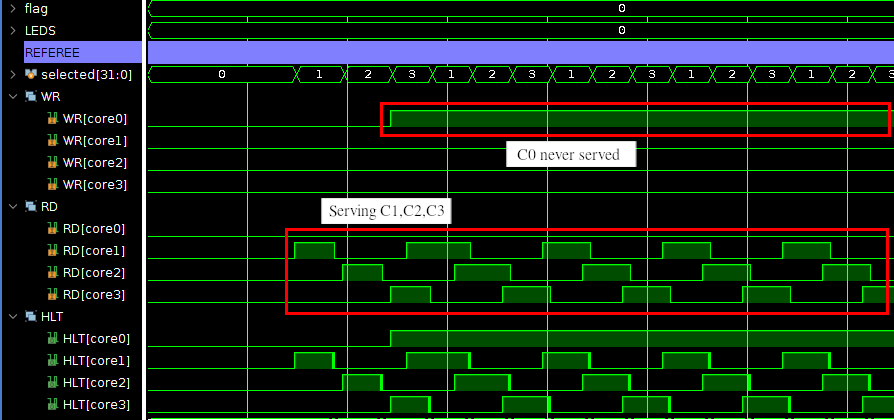
\includegraphics[width=1.0\textwidth]{images/flag4_sim_bad_crop_arrow.png}
    \caption{Simulation showing the memory hog problem.}
    \label{4LED-sim-bad}
\end{figure}

In Section~\ref{referee-behaviour} we mentioned that the \textit{Referee} prioritizes the core with the highest ID, if multiple were trying to access memory.
This explains what we see in Figure~\ref{4LED-sim-bad}.
At any point where the petition from core 0 is considered, a petition from a higher ID core is also active, so it does not get a chance to access memory.

To solve this, we changed how the served core is selected.
The \textit{Referee} has a register holding the prioritized core to serve.
It will always serve that core first if it is among the requesting cores when it receives multiple petitions.
If this is not the case, it selects the highest ID core from the rest.
After any petition, the register holding the prioritized core is increased.
This method ensures that all cores will get a chance to access memory, with a wait time of at most $N-1$ petitions in the worst case (i.e., when the core tries to access memory just after its turn has passed).

%figure showing this behavior?

After implementing this new logic, we simulated the same code from Figure~\ref{4LED-code} again and saw that everything was working as expected and the LEDs followed the desired pattern.

Finally, we tested a more realistic code.
We selected the \textit{dot product}, since it is really easily parallelized.
Remember that given two vector $v$ and $u$ of $n$ elements, the dot product is defined as $\sum_{i=0}^{n}{v_{i} * u_{i}}$.

In this case, we coded in C instead of in assembly to test how our design behaves when we do not manually pick the instructions but instead use a compiler.
The code follows these steps:
\begin{enumerate}
	\item Core 0 initializes the vectors to known values.
	\item All cores synchronize in a barrier.
	\item Every core computes its part of the sum ($\frac{n}{Ncores}$).
	\item In a reduction, each core accumulates its result in the same memory position.
\end{enumerate}

While most of the code can be done with plain C, we had to do some tweaks.
At the program's start, the stack pointer is manually set to an arbitrary position for each core, directly modifying the $sp$ register.
This is exemplified in Figure~\ref{stackfig}.

\begin{figure}[h!]
    \centering
    \begin{lstlisting}
asm volatile(
	"lui sp, 0x80000\t\n" //set up base stack
	"slli t0, tp, 7\t\n" //t0 = coreID*128
	"add sp, sp, t0\t\n" //sp = sp + t0;
);
    \end{lstlisting}
%    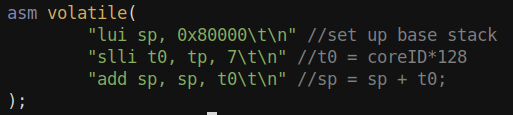
\includegraphics[width=.6\textwidth]{images/stack_ini.png}
    \caption{Initialization of the stack for multiple cores.}
    \label{stackfig}
\end{figure}

Furthermore, the global variables used to hold the vectors, synchronization flags, counters, and the final result are all pointers to an arbitrary position starting at 0x40000000, which is the start of the memory region to put the data.

The most interesting parts of the code are the barrier and the reduction, which work similarly.
In Figure~\ref{barrier} we show the code used for the barrier.

\begin{figure}[h!]
    \centering
    %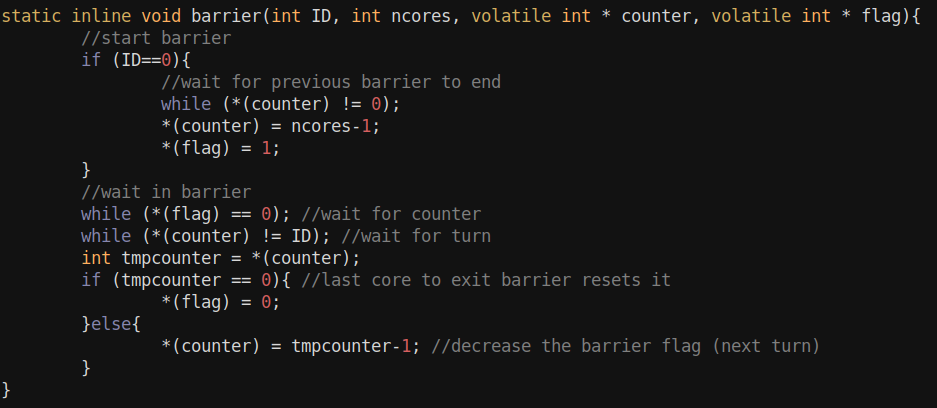
\includegraphics[width=.9\textwidth]{images/barrier.png}
    \begin{lstlisting}
static inline void barrier(int ID, int ncores, volatile int * counter, volatile int * flag){
	//start barrier
	if (ID==0){
		//wait for previous barrier to end
		while (*(counter) != 0);
		*(counter) = ncores-1;
		*(flag) = 1;
	}
	//wait in barrier
	while (*(flag) == 0); //wait for counter
	while (*(counter) != ID); //wait for turn
	int tmpcounter = *(counter);
	if (tmpcounter==0){//last core to exit barrier resets it
		*(flag) = 0;
	}else{
		*(counter) = tmpcounter-1; //decrease the barrier flag (next turn)
	}
}
    \end{lstlisting}
    \caption{Code snippet of the implemented barrier.}
    \label{barrier}
\end{figure}

Both are formed with a flag and a counter, which are both initialized at 0.
When core 0 arrives to the barrier, it sets the flag to 1 and sets the counter to $Ncores - 1$.
All cores except core 0 will wait until the flag is set and the counter equals their ID.
When that happens, they decrement the counter so the next core can do the same.
Then, the last core to exit the barrier resets it for future use.


The reduction works exactly the same, but with each core updating the content of the reduction variable when it is their turn.
It is important to note that in order for this code to work, each core has two registers hardcoded to its core ID and the total number of cores.


In Figure~\ref{4dot-sim} we see the simulation of the dot product with 4 cores.
We can see how core 0 initializes the vectors while the rest wait in the barrier until its flag is set to 1 and the counter decreases to 0.
Then, all cores compute their work, accessing their part of the vectors, and wait until core 0 starts the reduction.
Here, the same behavior as in the barrier is found until the correct result of 14 is generated.


\begin{figure}[h!]
    \centering
    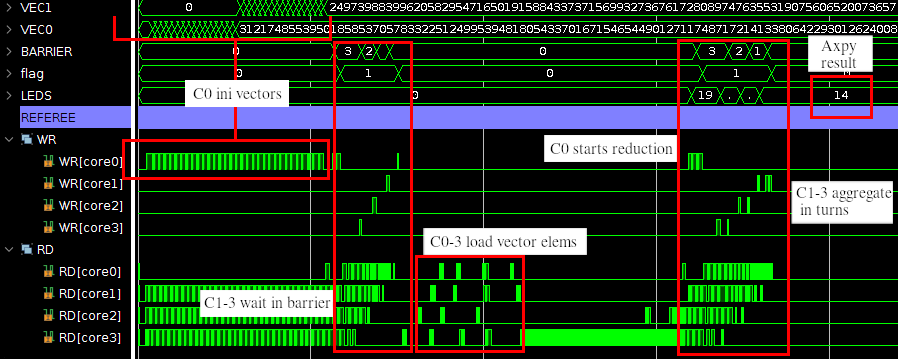
\includegraphics[width=1\textwidth]{images/axpy_sim4_crop_arrow.png}
    \caption{Simulation of the dot product with 4 cores.}
    \label{4dot-sim}
\end{figure}

We have also simulated it with 8 cores to show that the code is Ncores-agnostic, as can be seen in Figure~\ref{8dot-sim}.
The barrier and the reduction are longer, but the same result is obtained.

\begin{figure}[h!]
    \centering
    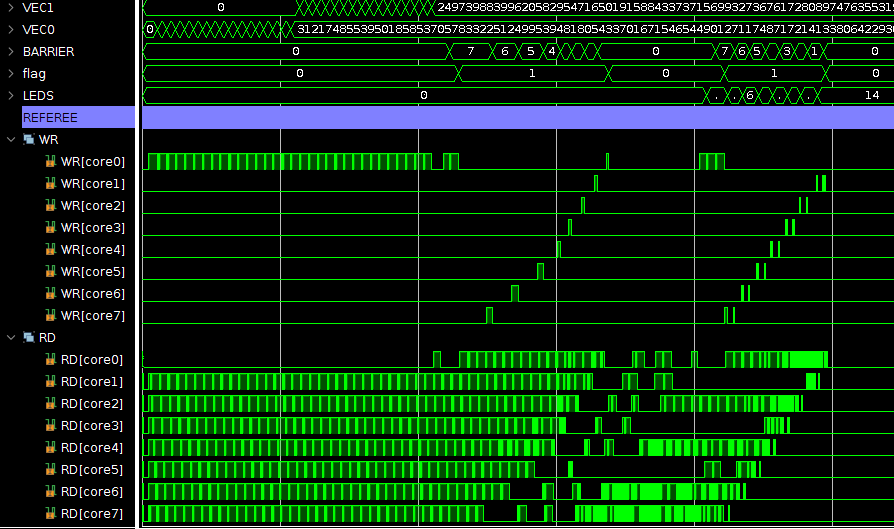
\includegraphics[width=.9\textwidth]{images/axpy_sim8_crop.png}
    \caption{Simulation of the dot product with 8 cores.}
    \label{8dot-sim}
\end{figure}












\section{\acrshort{ddr}}
\subsection{Justification}
After implementing and validating a multicore and referee design, the next step that we faced was replacing the \textit{fake} memory with the \gls{fpga}'s \gls{ddr}.

As mentioned in Section \ref{sec:fpga}, \gls{sp7} has an integrated \gls{ddr} memory of 4 Gb.
We wanted to connect our current dual-core \gls{rtl} to \gls{ddr} since memory was a one with dummy cycles to simulate memory delay. 
So, we would have not to simulate a memory, but to deal with a real one.


\subsection{Xilinx \acrshort{ip}}
Xilinx provides a \glspl{ip}, which are validated \gls{rtl} codes that ease the usage of a certain component from the \gls{fpga}. 
Usually, they implement the \gls{phy}, hiding the complexity and the specific implementation details of the component, and provide an standard interface to the programmer. 
This is very usefull because the \gls{phy} of a component can change from one \gls{fpga} to another, so having an standar user interface allows programmers to not worry that much when porting a design from one \gls{fpga} to another, which it is usually a not trivial process.

The \gls{ip} used for the \gls{ddr} is: \gls{mig} \cite{mig}.
This \gls{ip} is a controller and implementation of the \gls{phy} for interfacing user designs and provides an \gls{axi} slave interface.
Therefore, the chain is: an user design connected via \gls{axi} to the \gls{ddr} device.

\subsubsection{\acrshort{axi} protocol}
\acrlong{axi} is an standard industry protocol to connect different components in order to exchange data.
It is usually used as an information exchange protocol between logic blocks inside a complex digital circuit.
The \gls{axi} interface requieres a low number of resources and provides a great uniderectional data transfer bandwidth \cite{axi}.

We can see in Figure \ref{fig:axi} the \gls{axi} handshake. %with the minimum signals, more can be added to provide more information.
Data (\texttt{information}) won't be transmited until the sender has valid data (\texttt{tvalid}) and the receiver is ready (\texttt{tready}).
It is composed by a master interface and a slave interface.

\begin{figure}
    \centering
    %\includegraphics[width=0.7\textwidth]{../presentation/images/axi.png}
    \includegraphics[width=0.7\textwidth]{images/axi.png}
    \caption{\gls{axi} handshake.}
    \label{fig:axi}
\end{figure}

Information can be composed by many signal, the \texttt{data} one is the minimum one that has to be included.
Other signals can be added to \gls{axi} transactions in order to codify other information, such as the address.

\subsubsection{\acrshort{mig}}
As mentioned before, \gls{mig} provides an \gls{axi} interface to the programmer and is a customizable \gls{ip}. 
The most relevant options are the ones related to the \gls{axi} protocol, since they affect the \gls{rtl} design.
\begin{itemize}
    \item \texttt{ADDR\_WIDTH}: \\
        \gls{axi} address width for the slave and master interfaces. \\
        Options: up to 32 bits.
        
    \item \texttt{DATA\_WIDTH}: \\
        Width of the \gls{axi} read and write data for the slave and master interfaces. \\
        Options: 32, 64, 128, 256 bits.
\end{itemize}

The widths chosen are 32 bits for both options.

The \gls{mig} interface is the one that can be seen in Figure \ref{fig:mig}.
On the left side, there is the \gls{axi} interface to be connected with the user app. The left arrows indicate an input signal, and the right arrows an output.
On the right side, there is inputs/ouputs for the \gls{ddr} which are connected to the \gls{ddr} \gls{fpga}'s pins.

\begin{figure}
    \centering
    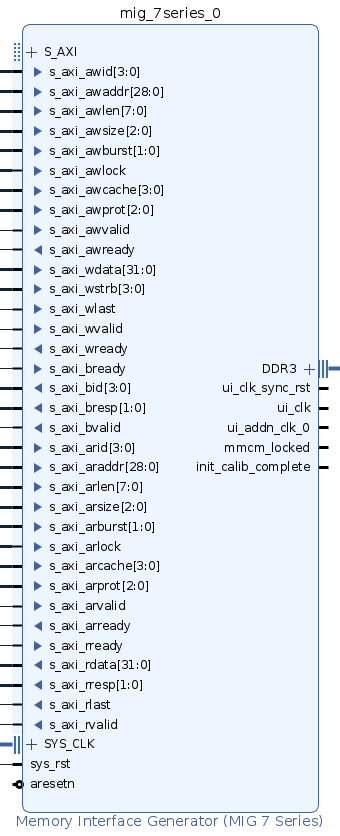
\includegraphics[width=0.55\textwidth]{images/mig_interface.png}
    \caption{\gls{mig} interface.}
    \label{fig:mig}
\end{figure}

\subsection{Implementation}
We implemented a \textit{bridge} to connect the \textit{referee} and the \gls{mig}.
It receives the transactions from the referee and refactors them into appropiated signals that the \gls{ddr} \gls{ip} needs. Also, a fine state machine was used to control the flow of the signals.

Therefore, the \gls{rtl} processor was modified in order to extract \gls{axi}'s \gls{mig} signals needed. 
The result is the block design that can be seen in Figure \ref{fig:bd_mig}, where our processors is connected to \gls{mig}.

    \begin{figure}
        \centering
        \makebox[\textwidth][c]{
        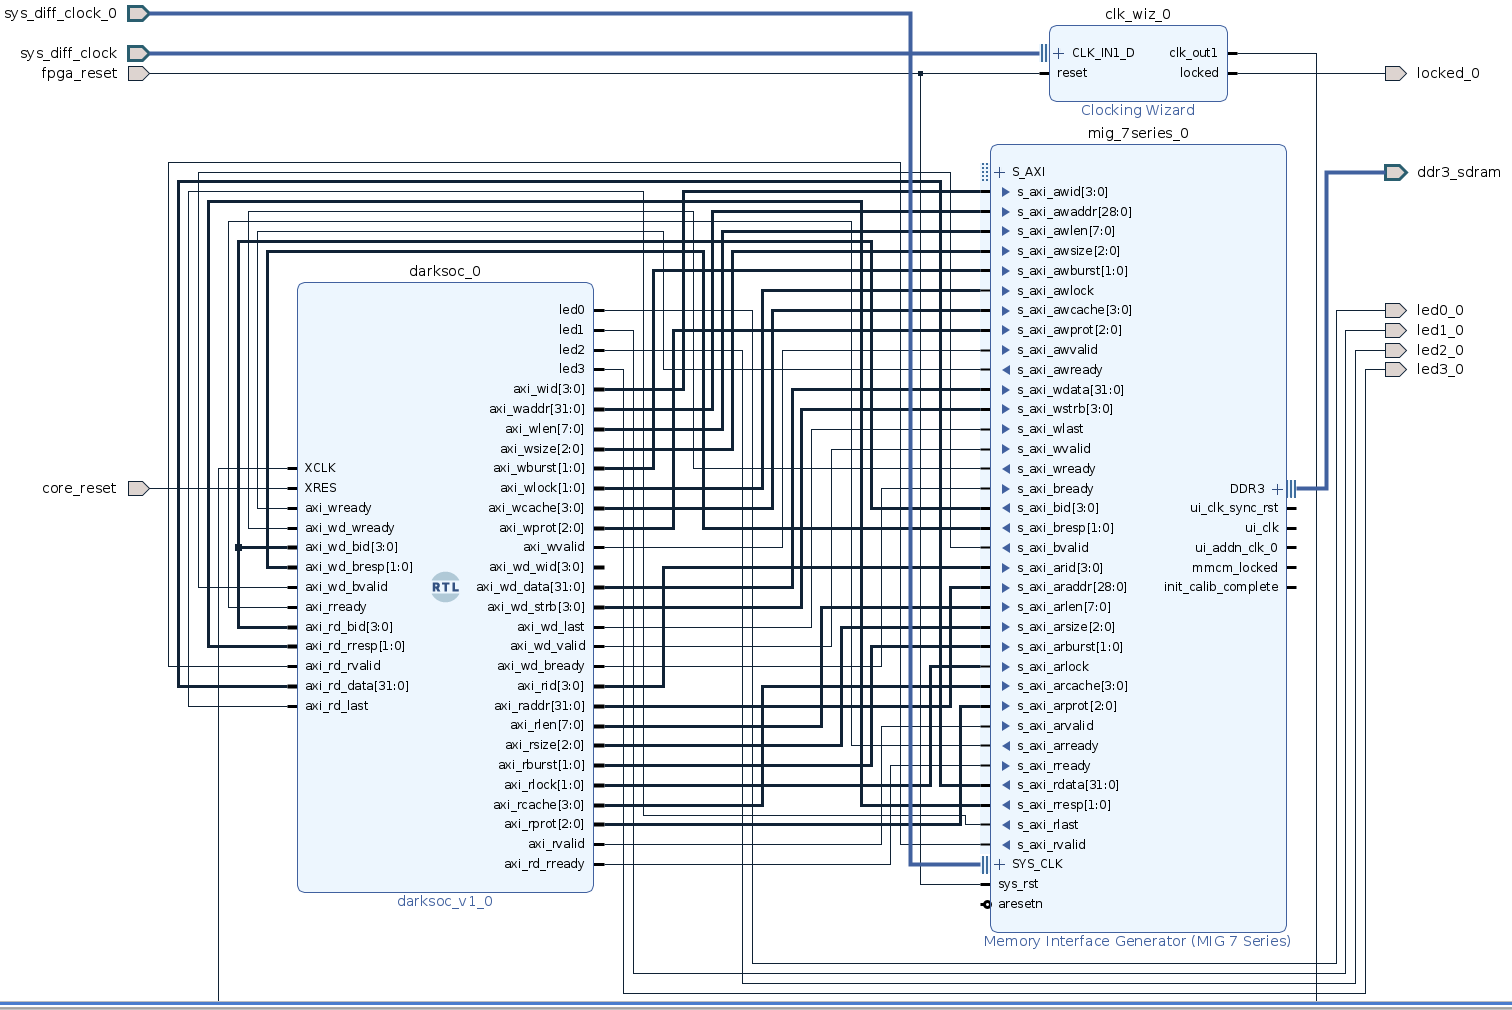
\includegraphics[width=1.2\textwidth]{images/bd_ddr.png}
        }
        \caption{Block design with \gls{mig}.}
        \label{fig:bd_mig}
    \end{figure}

\subsection{Validation}
The first validation step was with the Vivado simulator. 
\gls{mig} allows the simulation of the user app (our \gls{rtl} dual-core) and the \gls{ip} itself.

We adapted the testbench provided by Xilinx to connect our dual core. 
We ran the simulation and we detected that it was not simulating anything.
Some signals from the default waveform (the one provided in first intance by the \gls{ip} simulation) had a \texttt{Z} value, which means that they were not connected well.

We could not debbug the testbench in time.
The \gls{mig} testbench is a complex one, since it has to simulate the \gls{ddr}'s \gls{phy}, which is a tricky flow.

So, we could not proceed with the validation via simulation, and nor within the \gls{fpga}.




\begin{frame}{Conclusions}
    \begin{itemize}
        \item Followed a different path than the original
        \item RISC-V, multicore and boot
        \item Incremental steps
        \item Learnt to do an FPGA project from scratch
        \item Understood and implemented RTL
        \item Used Xilinx IPs
    \end{itemize}
\end{frame}



\bibliographystyle{unsrt}
\bibliography{../common/99_ref}
\end{document}
